\documentclass[a4paper,12pt]{article}
\usepackage[utf8]{inputenc}
\usepackage{graphicx}
\usepackage{subfig}
\usepackage{listings}
\usepackage{listingsutf8}
\usepackage{url}
\usepackage{amsmath}
%\title{TFG}
%\author{Miguel Ardura Zorita}
%\date{}
\usepackage{color}

\definecolor{mygreen}{rgb}{0,0.6,0}
\definecolor{mygray}{rgb}{0.5,0.5,0.5}
\definecolor{mymauve}{rgb}{0.58,0,0.82}

\lstset{ %
  backgroundcolor=\color{white},   % choose the background color; you must add \usepackage{color} or \usepackage{xcolor}
  basicstyle=\footnotesize,        % the size of the fonts that are used for the code
  breakatwhitespace=false,         % sets if automatic breaks should only happen at whitespace
  breaklines=true,                 % sets automatic line breaking
  captionpos=b,                    % sets the caption-position to bottom
  commentstyle=\color{mygreen},    % comment style
  deletekeywords={...},            % if you want to delete keywords from the given language
  escapeinside={\%*}{*)},          % if you want to add LaTeX within your code
  extendedchars=true,              % lets you use non-ASCII characters; for 8-bits encodings only, does not work with UTF-8
  frame=single,	                   % adds a frame around the code
  keepspaces=true,                 % keeps spaces in text, useful for keeping indentation of code (possibly needs columns=flexible)
  keywordstyle=\color{blue},       % keyword style
  language=Octave,                 % the language of the code
  otherkeywords={*,...},           % if you want to add more keywords to the set
  numbers=left,                    % where to put the line-numbers; possible values are (none, left, right)
  numbersep=5pt,                   % how far the line-numbers are from the code
  numberstyle=\tiny\color{mygray}, % the style that is used for the line-numbers
  rulecolor=\color{black},         % if not set, the frame-color may be changed on line-breaks within not-black text (e.g. comments (green here))
  showspaces=false,                % show spaces everywhere adding particular underscores; it overrides 'showstringspaces'
  showstringspaces=false,          % underline spaces within strings only
  showtabs=false,                  % show tabs within strings adding particular underscores
  stepnumber=2,                    % the step between two line-numbers. If it's 1, each line will be numbered
  stringstyle=\color{mymauve},     % string literal style
  tabsize=2,	                   % sets default tabsize to 2 spaces
  title=\lstname                   % show the filename of files included with \lstinputlisting; also try caption instead of title
}
\begin{document}
\lstset{inputencoding=utf8/latin1}
\renewcommand{\figurename}{Figura}
\begin{titlepage}
\begin{center}
\begin{figure}
\begin{center}
\includegraphics[width=8cm]{logo.jpg}
\end{center}
\end{figure}
FACULTAD DE CIENCIAS MATEMÁTICAS\\
\vspace{1cm}
\huge{\textbf{Técnicas de detección de galaxias en imágenes tomadas por telescopios por medio de Computer Vision}}\\
\vspace{3cm}
\rule{80mm}{0.1mm}\\
\begin{large}
Miguel Ardura Zorita\\
Director: Carlos Gregorio Rodríguez\\
\end{large}
\rule{80mm}{0.1mm}\\
\vspace*{0.1in}

\end{center}

\end{titlepage}

\newpage
\section*{Abstract}
This project addresses the detection of galaxies within a given raw telescope image. Since the input image comes with a high noise level, preprocessing steps are needed to successfully separate the interest regions, namely, the huge homogeneous pixel areas corresponding to galaxies and the small, isolated and highly illuminated pixel areas corresponding to stars. The detection of these two different objects, galaxies and stars, is carried out by means of two different processing paths, one for each object, and the outcome of them are images with the interest regions highlighted.
\\
\section*{Resumen}
Este proyecto aborda la detección de galaxias en una imagen sin procesar tomada por un telescopio. Puesto que las imágenes vienen con gran cantidad de ruido, se necesita preprocesarlas para poder diferenciar las zonas de interes, a saber, las grandes zonas homogéneas que corresponden a galaxias y las pequeñas y muy iluminadas zonas que corresponden a estrellas. La detección de estos dos tipos de objetos, galaxias y estrellas, es llevada a cabo por medio de dos caminos distintos, uno para cada objeto, y tienen como resultado imágenes con las zonas de interés destacadas.
\newpage
\renewcommand\contentsname{Índice general}
\tableofcontents
\newpage
\section{Motivación y objetivos}
Este trabajo tenía la tarea radical de servirme de una primera aproximación a la disciplina de la Visión Artificial. Si bien aquí se presenta una aplicación concreta al campo de la Astronomía, mi objetivo era conocer las técnicas utilizadas en la creación, manipulación y procesado de imágenes mediante las herramientas de que se dispone ahora, tanto de hardware como de software. La elección concreta de la Astronomía como campo de estudio surgió al poco de reunirme con mi tutor, Carlos Gregorio, y responde a mi afición por tal ciencia y deseo de poder experimentar con las imágenes generadas por los telescopios a un nivel superior al de un mero aficionado.
\\
Aunque en el camino se ha ido variando el rumbo del proyecto en multitud de ocasiones, finalmente decidí centrarlo en la detección semi-automática de galaxias tomando como input un fichero FITS\footnote{Ver la sección \ref{sec:FITS}} para una posterior clasificación en un trabajo futuro. El resultado del procesado es la detección de las estructuras candidatas a galaxias a través de sus contornos y la identificación de los objetos más brillantes de la imagen, con el fin de simplificar un trabajo posterior de discriminación de objetos no candidatos a galaxias.

\section{Librerías usadas}

En esta sección se informa brevemente de las herramientas que he utilizado a lo largo del proyecto, tanto los tipos de ficheros (FITS), como las librerías usadas (Astropy, OpenCV, Numpy, Matplotlib).
\subsection{Ficheros FITS}
\label{sec:FITS}

FITS\cite{fits} son las siglas de Flexible Image Transport System, un formato de archivo que sirve para recoger, transportar y procesar datos consistentes en arrays multidimensionales y tablas de metadatos. Surgió de la necesidad de disponer de un formato estándar con el que transferir datos astronómicos entre instalaciones cinentíficas.

En 1982 la Unión Astronómica Internacional (IAU por sus sigals en inglés) decidió respaldar formalmente este sistema de intercambio de datos, y desde su asamblea general de 1988 existe un comité derivado de su comisión de datos astronómicos que se encarga expresamente de mantener los estándares de FITS y revisar, aprobar y mantener su futuras extensiones, el IAU Working Group 

Un fichero FITS se compone de segmentos llamados HDU (Header/Data Unit). El primero es llamado 'Primary HDU', y generalmente consiste en un array que contiene un espectro de una dimensión, una imagen en dos dimensiones o un conjunto de datos en tres dimensiones.

Este HDU primario puede ir seguido de cualquier número de HDUs. Éstos se denominan \textit{extensiones} y actualmente pueden ser de tres tipos:
\begin{itemize}
\item Una imagen, consistente en array de píxeles de dimensión 0-999
\item Una tabla ASCII, que almacena información numérica en formato ASCII
\item Una tabla binaria, en cuyas celdas pueden almacenarse arrays 1-dimensionales siempre que las dimensiones en una misma columna de la tabla coincidan
\end{itemize}
Cada HDU consiste en un encabezado en formato ASCII (Header Unit) seguido de una sección opcional que almacena el array de píxeles de la imagen (Data Unit). Cada Header Unit contiene una secuencia de claves con sus valores correspondientes con el siguiente formato
\begin{center}
CLAVE = valor / comentario en forma de string
\end{center}
En estas claves se almacena, entre otros, información sobre las características del telescopio que tomó la imagen, coordenadas de la región a la que se apuntaba en el momento de producirse la observación y dimensiones y formato de la imagen generada.
Por otro lado, los píxeles de la imagen almacenada en el Primary HDU o en las eventuales extensiones de tipo imagen, serán de uno de los cinco siguientes tipos actualmente soportados: enteros sin signo 8-bit, enteros con signo 16-bit, enteros con signo 32-bit, 32-bit IEEE float y 64-bit IEEE float.

Las imágenes usadas en este trabajo vienen almacenadas en el HDU primario y son 2-dimensionales y float 32. En el código adjunto imageInfo.py se muestra el contenido de los HDU del fichero frame-i-002830-6-0398.fits, usado a lo largo de esta memoria.
\subsubsection{Astropy}
Para poder interactuar con los ficheros FITS a través de Python he usado el paquete \textbf{astropy.io.fits} de la librería Astropy\cite{astropy}, que es un proyecto libre escrito en Python y diseñado para trabajar en Astronomía.

Este paquete es de un manejo sencillo y su uso se muestra en la sección \ref{sec:Procesado}.
\subsection{OpenCV}
OpenCV\cite{opencv,oreilly} es una librería multiplataforma de código abierto escrita en C y C++ que permite trabajar con imágenes y visión artificial. Surgió originariamente en 1999 como un proyecto de Intel para mejorar el rendimiento de la CPU y ejecuciones en tiempo real y actualmente cuenta con más de 2500 algoritmos específicos de \textit{computer visión} optimizados, abarcando tareas como el reconocimiento de objetos en imágenes y vídeos, el seguimiento de objetos en vídeo, comparación de imágenes con una base de datos dada, procesado de imágenes para mejorar su calidad, o incluso extraer modelos 3d de objetos. Tiene una comunidad de más de 47.000 usuarios, más de 7 millones de descargas y es actualmente usada por empresas privadas, grupos de investigación e incluso gobiernos. Su desarrollo actual está dirigido por Itseez.

En este trabajo se usa la versión 2.4 de la API para Python.
\subsection{NumPy}
NumPy\cite{numpy} es una librería de código abierto resultado de la mejora de en 2005 de la reescritura de Numeric por parte de Travis Oliphant. Es una librería que permite trabajar con arrays multidimensionales e incorpora gran cantidad de funciones de alto nivel sobre estos arrays.
\section{Desarrollo del proyecto}
\label{sec:desarrollo}
\subsection{Procesado de los ficheros FITS}
\label{sec:Procesado}
El proceso de tratado de las imágenes empieza con la carga y lectura de los ficheros FITS. Esto se hace por medio de la librería Astropy. Como se explica en la sección \ref{sec:FITS}, la matriz que representa la imagen que se usará aquí se corresponde con el primer HDU. Así, el siguiente código carga en 'img' el ndarray de numpy contenido en el archivo FITS de muestra:

\lstinputlisting[language=Python, frame= single, firstline=1, lastline=5]{basicLoading.py}

El siguiente código hace uso de OpenCV para mostrar la imagen antes cargada. Se realiza un mapeo lineal de los valores leídos del FITS a [0,1] para normalizar los valores de la imagen y que la función \textbf{imshow} no aparezca en blanco debido a la conversión al rango [0,255] que \textbf{imshow}\cite{imshow} realiza a las imágenes en float 32:

\lstinputlisting[language=Python, firstline=7]{basicLoading.py}

La figura \ref{fig:img1} muestra la imagen cargada con el script anterior.
\begin{figure}[h!]
\centering
\fbox{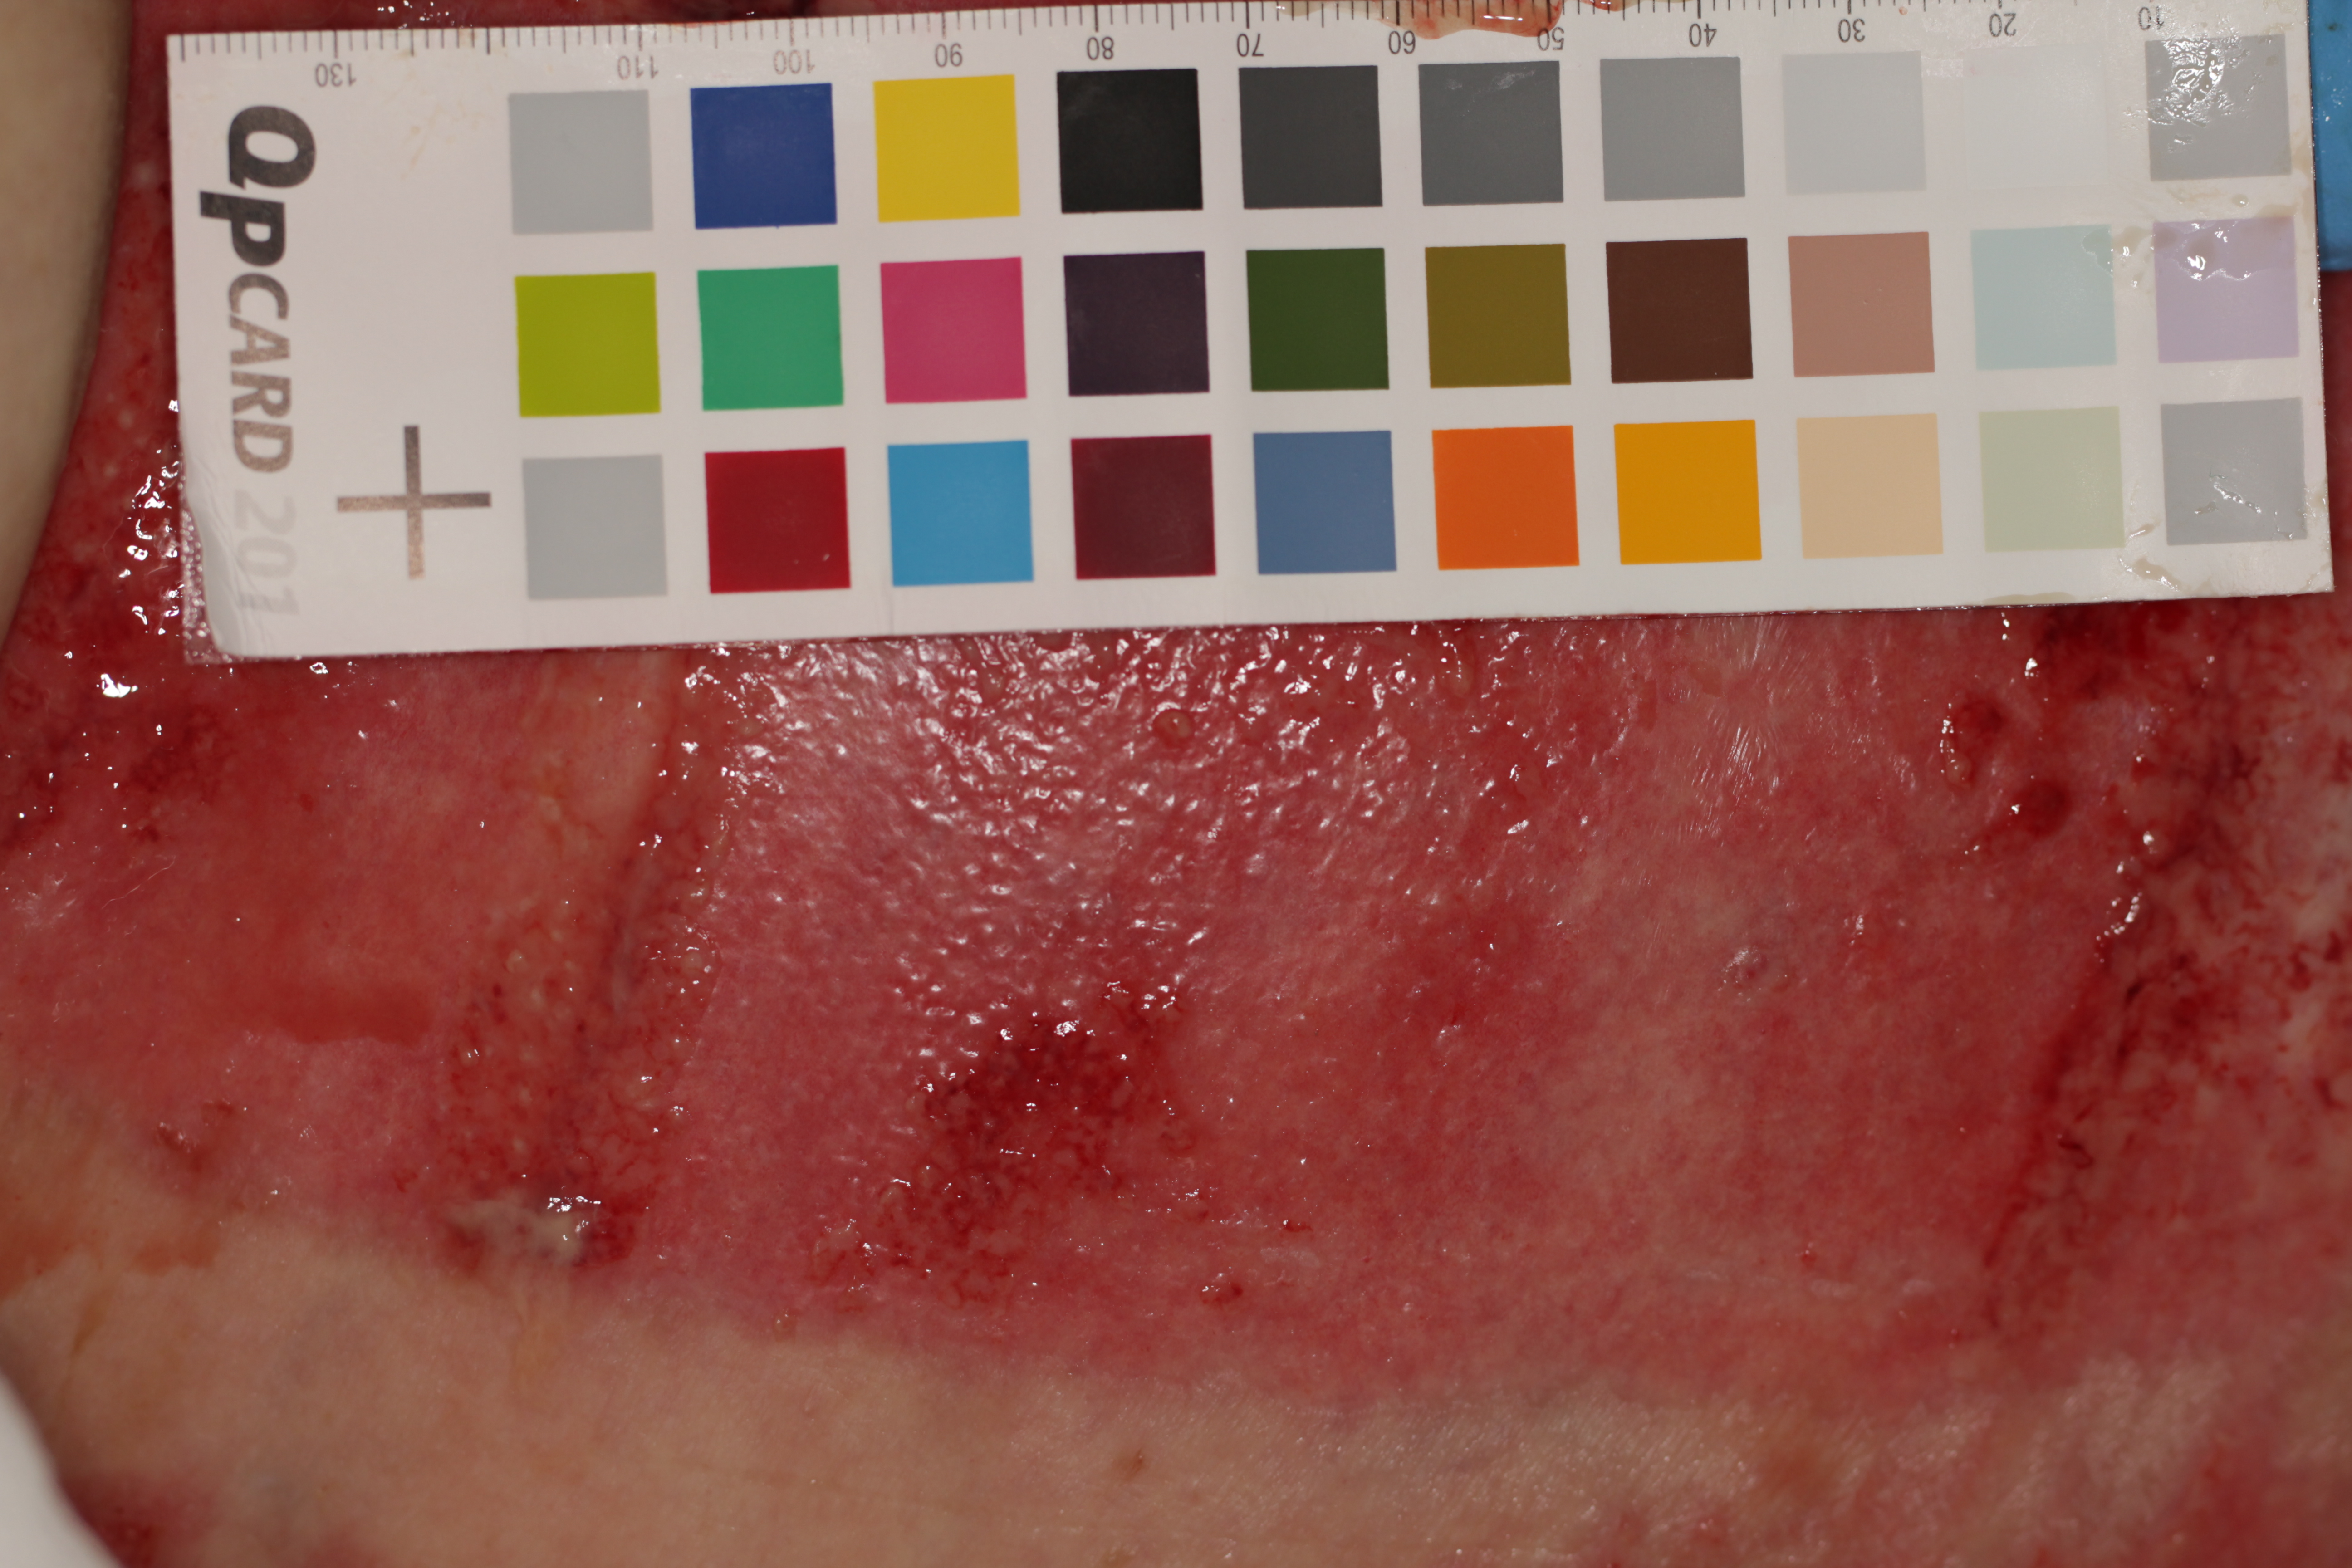
\includegraphics[width=10cm]{img1.png}}
\caption{Visualización del archivo frame-i-002830-6-0398.fits por medio de \textit{basicLoading.py}.}
\label{fig:img1}
\end{figure}

\subsection{Detección de los candidatos a galaxia}
A lo largo de esta sección se muestran los dos caminos seguidos para extraer la información sobre el contenido de la imagen con el fin de detectar galaxias y estrellas que contenga.
\subsubsection{Procesado inicial: eliminación de ruido y estrellas menos luminosas}

Ante la problemática surgida en lo que respecta a la eliminación del ruido de las imágenes haciendo uso de las herramientas predefinidas en la librería OpenCV (como se muestra en la sección \ref{sec:Problemas}), creé un filtro con el que obtengo resultados más cercanos a lo que quería. En concreto consiste en el uso del método \textbf{filter2D}\cite{filter2d} de OpenCV. Dicho método sirve para crear un filtro a partir de un una matriz dada.

La aplicación de un filtro a una imagen consiste principalmente en la combinación de una matriz, llamada kernel en este contexto, con la imagen original por medio de una convolución. Una convolución es una operación que consiste en combinar los valores del kernel con secciones de la imagen de igual dimensión para obtener unos nuevos valores para los píxeles de la imagen. Partiendo de una imagen y un kernel con uno de sus elementos marcado como \textit{pivote}, el proceso es el siguiente:

\begin{enumerate}
\item Se superpone el elemento pivote del kernel con un píxel de la imagen original, con los elementos del resto del kernel superpuestos a los correspondientes píxeles de la imagen.
\item Se multiplican los coeficientes del kernel por el valor de los píxeles correspondientes de la imagen y se suma el resultado.
\item El resultado anterior se fija como nuevo valor del píxel de la imagen sobre el que se situó el pivote.
\item Se repiten los puntos 1, 2 y 3 para el resto de píxeles de la imagen original.
\end{enumerate}

El resultado es una nueva imagen en la que los valores de los píxeles dependen tanto de los coeficientes del kernel como de la imagen anterior. Es por esto por lo que los filtros vienen dados principalmente por el kernel que los representa.

En concreto, creé el kernel
$\begin{pmatrix}
0 & 1 & 0 \\
1 & 0 & 1 \\
0 & 1 & 0
\end{pmatrix}$
después de observar que el intenso granulado innato de las imágenes que tomaba de los FITS hacía que al aplicar los filtros predefinidos de OpenCV el resultado fuera una imagen con gran cantidad de ruido añadido. Intentando destacar regiones luminosas y no tanto conservar las pequeñas regiones de pocos píxeles, decidí ponderar solo los píxeles de alrededor (arriba, abajo, izquierda y derecha) en lugar de considerar más píxeles vecinos, que era lo que añadía el ruido en el caso de los otros filtros.

Tomando la imagen resultado de aplicar este filtro a la imagen leída de los archivos FITS, y aplicando técnicas de segmentación, obtuve resultados con los que pude seguir avanzando.

\subsubsection{Destacando formas de galaxias con segmentación}

Me encontré con que, junto con la aplicación del filtro que creé, las técnicas de segmentación de las que provee OpenCV eran suficiente para eliminar gran cantidad del ruido existente en las imágenes. Esto me es de gran utilidad en el proceso de la detección de galaxias porque reduce enormemente la cantidad de información no útil para este propósito, como las regiones vacías o en las que los objetos luminosos no aparecen agrupados de forma ordenada.

En concreto uso el método de \textit{thresholding}, que es una técnica de segmentación que consiste en una identificación de los valores de la imagen a través de una relación de equivalencia dada. En términos de Teoría de Conjuntos esto equivale a la construcción del espacio cociente del conjunto de píxeles por medio de la relación de equivalencia que dicte el método, y en el que a los píxeles relacionados se les asignará el mismo valor en el espacio cociente resultante.

Tales relaciones son, en el caso de segmentación por \textit{thresholding}\cite{threshold}, de comparación con un umbral dado. OpenCV ofrece cinco tipos de segmentación usando este método (ver \ref{sec:thresh}).

El que me daba mejores resultados y decidí usar es el binario invertido.

En lo que respecta a los parámetros de la función, encontré que el umbral obtenido automáticamente por el algoritmo de Otsu\cite{otsu} y el valor máximo igual a 1 daban los resultados más aproximados a lo que buscaba.
El siguiente código recoge la aplicación de esto anterior:
\lstinputlisting[language=Python]{customFilter+thresholding.py}
y la figura \ref{fig:img2} muestra la imagen que es generada por el código anterior a partir de la imagen antes vista.

\begin{figure}[!h]
\centering
\fbox{\includegraphics[width=8cm]{img2.png}}
\caption{Imagen resultado de aplicar lo anterior a la imagen vista antes.}
\label{fig:img2}
\end{figure}

Como se puede observar, gran parte del granulado de la imagen original ha desaparecido y en su lugar se distinguen motas aisladas y una gran estructura. Se aprecia claramente una zona central de la que salen brazos finos hacia el exterior.

A fin de conseguir que esta detección fuera automática, introduje el estudio de \textit{contornos} en la imágenes obtenidas, lo que lleva a la siguiente etapa del procesado.

\subsubsection{Detección de las galaxias a través de sus contornos}
Con el fin de identificar y aislar las regiones oscuras que aparecen aplicando \textit{thresholding}, incorporo el uso del método de OpenCV que detecta contornos, \textbf{findContours}\cite{findcontours}. Esta función toma como input una imagen de 8 bits, un modo y un método y devuelve la lista de contornos. Como modo utilizo el que devuelve los contornos en una estructura anidada (\textbf{RETR\_TREE}), y como método de aproximación de los contornos, uso el que comprime los segmentos para almacenar solo sus extremos (\textbf{CHAIN\_APPROX\_SIMPLE}). El objetivo es usar el método de OpenCV que determina el rectángulo que se ajusta a cada contorno, y entre todos esos rectángulos quedarse con el de mayor área, que es el que contiene al contorno candidato a estructura de interés. Para esto hago uso del método \textbf{boundingRect}\cite{boundingrect}, que dado un contorno, devuelve cuatro parámetros que corresponden a las dos coordenadas del vértice superior izquierdo, la base y la altura del rectángulo horizontal que ajusta al contorno.


El siguiente script muestra su uso:
\lstinputlisting[language=Python]{contours+BoundingRects.py}
y la figura \ref{fig:img3} muestra la imagen resultante.

\begin{figure}[!h]
\centering
\fbox{\includegraphics[width=8cm]{img3.png}}
\caption{Rectángulos ajustando los contornos.}
\label{fig:img3}
\end{figure}
Para determinar el rectángulo de mayor área, se predefine un rectángulo inicial de alto y ancho iguales a cero para en cada iteración sobre los contornos comparar el rectángulo que ajusta al contorno de la iteración con el de máximo área actual. Se corresponde con la siguiente sección del código:
\lstinputlisting[language=Python, frame= single, firstline=25, lastline=29]{contours+BoundingRects.py}
La condición $w*h<2040*1480$ descarta el contorno que corresponde al borde exterior de la imagen, pues eventualmente puede aparecer como resultado del cálculo de contornos.

La figura \ref{fig:img3Rect} muestra el resultado de recortar la imagen \ref{fig:img3} por el rectángulo de mayor área detectado.

\begin{figure}[!h]
\centering
\fbox{\includegraphics[width=4cm]{img3Rect.png}}
\caption{Recorte del contorno identificado.}
\label{fig:img3Rect}
\end{figure}


\subsection{Detección de candidatos a estrellas}
Con el fin de identificar todas las posibles galaxias presentes en la imagen, surge la necesidad de determinar cuándo una región luminosa se corresponde con una estrella y cuándo con una galaxia, pues ambos objetos pueden presentar tamaños y formas similares.

A diferencia de la discretización anterior, me centro ahora en la identificación de los objetos que por su luminosidad se destacan sobre su alrededor. Para ello hago un uso combinado del filtro customizado y función de \textit{thresholding} antes mencionados, y lo combino con la función \textbf{morphology}\cite{morphologyex} de OpenCV, que proporciona herramientas para el uso de transformaciones morfológicas.

Una transformación morfológica es básicamente una operación que provee de información sobre la estructura de una imagen por medio de la aplicación de un elemento estructurador. Generalmente consistirá en la convolución de la imagen de partida con un kernel. La naturaleza de este kernel será lo que determine la imagen resultado.

Las transformaciones implementadas disponibles en \textbf{morphology} se basan en dos operaciones básicas: la \textit{dilatación} y la \textit{erosión}. En ambos casos se convoluciona con un kernel que generalmente tiene forma rectangular o circular y a cada píxel se le asigna un nuevo valor dependiendo de los valores de los píxeles que lo rodeen . En el caso de la dilatación se toma el máximo valor de los píxeles del entorno definido por el kernel, y en el caso de la erosión el mínimo. Cuando la imagen es binaria estos valores se corresponden con 1 y 0 respectivamente.

Combinando estas dos transformaciones, OpenCV provee de varias operaciones de segmentación (ver el apéndice \ref{sec:morph}).
A través de la experimentación encontré que la operación cierre conseguía descartar la mayor cantidad de ruido de la mayoría de las imágenes, salvo en algunos casos, en los que por la naturaleza de las imágenes los procedimientos aquí usados dan resultados erróneos (véase sección \ref{sec:Problemas}.

El siguiente código muestra el uso de la operación cierre:
\lstinputlisting[language=Python, firstline=1, lastline=16]{blobDetection.py}
y la figura \ref{fig:img4} muestra la imagen resultante de aplicar en cinco iteraciones la operación cierre.
\begin{figure}[h!]
\centering
\fbox{\includegraphics[width=8cm]{img4.png}}
\caption{Operación cierre.}
\label{fig:img4}
\end{figure}

Una vez que se tiene una imagen binaria y con solo los elementos más brillantes de la imagen original, creé un detector de \textit{blobs}, como se explica en la siguiente sección.

\subsubsection{Blob detection}

Un \textit{blob} es un grupo de píxeles de una imagen que comparten la propiedad de tener valores similares. En la figura \ref{fig:img4} cada región oscura aislada es un \textit{blob}, y el objetivo de esta sección es detectarlos.

En OpenCV se dispone de la función \textbf{SimpleBlobDetector} para lograr esto. Basta con fijar una serie de parámetros que se refieren a unas características básicas (a saber: color, tamaño y forma).

El siguiente código muestra el detector de \textit{blobs} que creé y los parámetros con los que obtuve mejores resultados, que son una convexidad mínima de 0.5 y un valor de la elongación mínimo de 0.1:

\lstinputlisting[language=Python, firstline=21]{blobDetection.py}
y la figura \ref{fig:img5} muestra el resultado de aplicar el detector de \textit{blobs}.
\begin{figure}[h!]
\centering
\fbox{\includegraphics[width=8cm]{img5.png}}
\caption{Detección de \textit{blobs}.}
\label{fig:img5}
\end{figure}

En la figura \ref{fig:img6} se ve en detalle una región de la imagen \ref{fig:img5}.
\begin{figure}[h!]
\centering
\fbox{\includegraphics[width=5cm]{img5Zoom.png}}
\caption{Detección de \textit{blobs} en detalle.}
\label{fig:img6}
\end{figure}

\section{Problemas encontrados}
\label{sec:Problemas}
A la hora de realizar este trabajo me he encontrado principalmente con dos problemas. El primero es la falta de imágenes con las que trabajar y sobre todo de calidad adecuada para trabajar con ellas a nivel amateur-académico iniciado. Si bien se pueden encontrar muchos sitios web con ficheros FITS de acceso libre tras buscar un poco en Internet, pocos eran los que disponían de una base de datos que alguien profano en la materia pudiera entender y manejar con soltura en un primer acercamiento al manejo de los mismos.

Finalmente di con el sitio web de un proyecto que libera ficheros FITS etiquetados por su contenido, lo que me resultó muy útil para acceder de manera directa a imágenes de galaxias, a fin de empezar a trabajar con ellas. Este sitio es "The Sloan Digital Sky Survey: Mapping the Universe" (www.sdss.org). Lamentablemente para mí, el buscador interno de la página dejó de funcionar y tuve problemas para conseguir nuevos ficheros con los que trabajar.

El segundo problema es la naturaleza de las imágenes captadas por los telescopios. Al ser el principal objetivo del trabajo aprender a usar OpenCV, intenté primero obtener resultados haciendo uso de sus funciones predefinidas, pero me encontré con que parecían estar hechas principalmente para su aplicación en imágenes tomadas en el espectro visible. Las imágenes astrónomicas obtenidas de los ficheros FITS distan mucho de ser tan nítidas como las obtenidas por cualquier cámara de fotos, y si se representan tal y como son leídas directamente del FITS, probablemente no se distingan nada más que gránulos grises. Esto es de esperar, puesto que no están hechas para ser mostradas, al menos en crudo, pero explica por qué necesité crear mi propio filtro para obtener algún resultado. Una vez superado esto pude satisfactoriamente hacer uso de las funciones de OpenCV.



\section{Conclusión y trabajo futuro}
En resumen, se han definido métodos para, partiendo de una imagen de un fichero FITS, identificar tanto las grandes regiones luminosas candidatas a galaxias como objetos más brillantes de la imagen. El siguiente paso sería continuar con la clasificación de las imágenes ya simplificadas y separadas en sus zonas de interés. Esto se podría hacer de varias maneras. Por ejemplo, si se dispusiera de una gran base de datos con ficheros FITS etiquetados por los objetos astronómicos que contienen, se podrían usar técnicas de Machine Learning para crear clasificadores automáticos con ajuste dinámico de los parámetros de todas las funciones usadas. Esto serviría para salvar el inconveniente de la gran disparidad de las imágenes, que lleva a la necesidad de ajustar para cada imagen los valores de los parámetros usados para realizar una clasificación satisfactoria.


\appendix
\section{Apéndices}
\subsection{Detalle de las opciones de thresholding y morphology}
\subsubsection{Thresholding}
\label{sec:thresh}
Los cinco tipo de segmentación aplicables en el método \textbf{thresholding} son:
\begin{itemize}
\item \textbf{Binario:} Fijado un umbral, si el valor de un píxel excede ese umbral, se le asigna un valor fijado como máximo; si no, se le asignará 0.
\item \textbf{Binario invertido:} Análogo al anterior, pero con las condiciones invertidas.
\item \textbf{Truncado:} Si el valor de un píxel excede el umbral, se le asignará el umbral como nuevo valor. En caso contrario no se ve alterado.
\item \textbf{Truncado a cero:} Si el valor de un píxel es menor que el del umbral, se le asigna el valor cero. En caso contrario no se ve alterado.
\item \textbf{Truncado a cero invertido:} Análogo al anterior, pero con las condiciones invertidas.
\end{itemize}
\subsubsection{Morphology}
\label{sec:morph}
El método \textbf{morphology} dispone de las siguientes operaciones morfólogicas:
\begin{itemize}
\item \textbf{Apertura (open): } es el resultado de aplicar una erosión seguida de una dilatación.
\begin{center}
$apertura(imagen, kernel) = dilataci\acute{o}n(erosi\acute{o}n(imagen,kernel), kernel)$
\end{center}
\item \textbf{Cierre (close):} es el resultado de aplicar una dilatación seguida de una erosión.
\begin{center}
$cierre(img, kernel) = erosi\acute{o}n(dilataci\acute{o}n(imagen,kernel),kernel)$
\end{center}
\item \textbf{Gradiente:} es la diferencia de la erosión y la dilatación de una imagen.
\begin{center}
$gradiente(imagen, kernel) = dilataci\acute{o}n(imagen,kernel) - erosi\acute{o}n(imagen,kernel)$
\end{center}
\item \textbf{Top Hat:} es la diferencia de la imagen inicial y su apertura.
\begin{center}
$tophat(imagen, kernel) = imagen - apertura(imagen, kernel)$
\end{center}
\item \textbf{Black Hat:} es la diferencia del cierre y la imagen inicial.
\begin{center}
$blackhat(imagen, kernel) = cierre(imagen, kernel)- imagen$
\end{center}
\end{itemize}

En el script morphExample.py se puede ver el efecto de estas operaciones morfólogicas.



\subsection{Muestras del procesado de otras imágenes}
Las figuras \ref{fig:img7}, \ref{fig:img8}, \ref{fig:img9}, \ref{fig:img10} \ref{fig:img11}, \ref{fig:img12} y \ref{fig:img13} muestran el resultado de aplicar a otras imágenes obtenidas de ficheros FITS los mismo procedimientos que se han mostrado a lo largo del punto \ref{sec:desarrollo}. Se observa cómo de algunas imágenes se obtienen resultados espurios fruto de la necesidad de ajustar los parámetros de algunas funciones casi de manera independiente por la naturaleza de esas imágenes. Se pueden ver ejemplos de este ajuste dinámico, material del trabajo que seguiría al descrito aquí, en los scripts adjuntos.
\begin{figure}[htbp!]
\centering
\subfloat[Imagen base.]{\fbox{\includegraphics[width=12.2cm]{1.png}}}\\
\subfloat[\scriptsize{Detección de la galaxia por su contorno.}]{\fbox{\includegraphics[width=6.1cm]{GG1.png}}}\hspace{0.5cm}
\subfloat[\scriptsize{Detección de las estrellas más luminosas.}]{\fbox{\includegraphics[width=6.1cm]{GG1'}}}
\caption{Galaxia m81.}
\label{fig:img7}
\end{figure}

\begin{figure}[htbp!]
\centering
\subfloat[Imagen base.]{\fbox{\includegraphics[width=12.2cm]{2.png}}}\\
\subfloat[\scriptsize{Detección de la galaxia por su contorno.}]{\fbox{\includegraphics[width=6.1cm]{GG2.png}}}\hspace{0.5cm}
\subfloat[\scriptsize{Detección de las estrellas más luminosas.}]{\fbox{\includegraphics[width=6.1cm]{GG2'}}}
\caption{Galaxia m66.}
\label{fig:img8}
\end{figure}

\begin{figure}[htbp!]
\centering
\subfloat[Imagen base.]{\fbox{\includegraphics[width=12.2cm]{3.png}}}\\
\subfloat[\scriptsize{Detección de la galaxia por su contorno.}]{\fbox{\includegraphics[width=6.1cm]{GG3.png}}}\hspace{0.5cm}
\subfloat[\scriptsize{Detección de las estrellas más luminosas.}]{\fbox{\includegraphics[width=6.1cm]{GG3'}}}
\caption{Galaxia m91.}
\label{fig:img9}
\end{figure}

\begin{figure}[htbp!]
\centering
\subfloat[Imagen base.]{\fbox{\includegraphics[width=12.2cm]{4.png}}}\\
\subfloat[\scriptsize{Detección de la galaxia por su contorno.}]{\fbox{\includegraphics[width=6.1cm]{GG4.png}}}\hspace{0.5cm}
\subfloat[\scriptsize{Detección de las estrellas más luminosas.}]{\fbox{\includegraphics[width=6.1cm]{GG4'}}}
\caption{Galaxia m59.}
\label{fig:img10}
\end{figure}

\begin{figure}[htbp!]
\centering
\subfloat[Imagen base.]{\fbox{\includegraphics[width=12.2cm]{5.png}}}\\
\subfloat[\scriptsize{Detección de la galaxia por su contorno.}]{\fbox{\includegraphics[width=6.1cm]{GG5.png}}}\hspace{0.5cm}
\subfloat[\scriptsize{Detección de las estrellas más luminosas.}]{\fbox{\includegraphics[width=6.1cm]{GG5'}}}
\caption{Galaxia m33.}
\label{fig:img11}
\end{figure}

\begin{figure}[htbp!]
\centering
\subfloat[Imagen base.]{\fbox{\includegraphics[width=12.2cm]{6.png}}}\\
\subfloat[\scriptsize{Detección de la galaxia por su contorno.}]{\fbox{\includegraphics[width=6.1cm]{GG6.png}}}\hspace{0.5cm}
\subfloat[\scriptsize{Detección de las estrellas más luminosas.}]{\fbox{\includegraphics[width=6.1cm]{GG6'}}}
\caption{Galaxia m74.}
\label{fig:img12}
\end{figure}

\begin{figure}[htbp!]
\centering
\subfloat[Imagen base.]{\fbox{\includegraphics[width=12.2cm]{7.png}}}\\
\subfloat[\scriptsize{Detección de la galaxia por su contorno.}]{\fbox{\includegraphics[width=6.1cm]{GG7.png}}}\hspace{0.5cm}
\subfloat[\scriptsize{Detección de las estrellas más luminosas.}]{\fbox{\includegraphics[width=6.1cm]{GG7'}}}
\caption{Galaxia m95.}
\label{fig:img13}
\end{figure}

\subsection{Trabajo descartado}
Esta sección contiene el trabajo realizado pero no utilizado por no proporcionar los resultados que buscaba. %\cite{test}
\subsubsection{Sobel}
En el script SobelExample.py se puede ver el resultado de aplicar el operador Sobel. No lo usé porque no conseguía eliminar el ruido y la forma de la galaxia resultaba demasiado alterada.
\subsubsection{Flow}
El script flowExample.py muestra el resultado de aplicar el método cornerEigenValsAndVecs, que sirve para determinal esquinas en las imágenes por medio de autovalores y autovectores. No lo usé porque no destacaba suficiente la forma de la galaxia sobre el resto de la imagen.
\subsubsection{Canny}
En el script CannyExample.py se muestra el resultado de aplicar el algoritmo de Canny para detectar aristas. No lo usé porque al necesitar preprocesar la imagen base para usarla como input del método Canny, se producía un ruido que producía resultados no deseados.
\subsubsection{3d}
En el script 3dExample.py se muestra un primer acercamiento a la clasificación de los objetos en la imagen por medio de su visualización 3d. Lo acabé descartando porque la enorme dimensión de las imágenes de los ficheros FITS superaba la capacidad de los equipos en los que he trabajado y no pude avanzar en ese sentido.

\addcontentsline{toc}{section}{Bibliografía y referencias}
\renewcommand\refname{Bibliografía y referencias}
\bibliographystyle{unsrt}
\bibliography{biblio}
%\nocite{*}
%\listoffigures
%\listoftables

\end{document}
